\section{Introduction}
\label{sect:intro}

Prostate-specific membrane antigen (PSMA) PET/CT is now routinely used for staging prostate cancer, for planning and following radioligand therapy, and for assessing treatment response~\cite{ref_psma_clinical}.
In such longitudinal imaging, patients are scanned before therapy (baseline) and again at one or more follow-up time points.
Registering each follow-up image to the baseline image makes it possible to compare tumor burden voxel by voxel or track individual lesions over time~\cite{ref_psmareg_challenge}.
For these uses, a registration has to align the anatomy while preserving the PET-derived quantities of the warped image.
Two such quantities, under the names used by the Learn2Reg 2026 PSMAReg challenge~\cite{ref_psmareg_challenge}, are the metabolic tumor volume (MTV) and the total lesion glycolysis (TLG); for PSMA PET, they measure the PSMA-positive tumor volume and the total lesion PSMA uptake.
A deformation that compresses or stretches a lesion would change both these quantities and thereby introduce a registration-induced bias into the measured longitudinal change.
When the registered follow-up is used to match lesions or compare them with baseline, such processing-induced changes could be mistaken for part of the longitudinal change and could therefore affect lesion tracking or response assessment.
The challenge, part of the Learn2Reg series~\cite{ref_learn2reg_hansen,ref_learn2reg_alessa} and based on the PSMA-PET-CT-Lesions dataset~\cite{ref_psmaregdata}, formalizes this setting by registering each follow-up image to its baseline image with a dense deformation field.
It scores organ overlap, boundary distance, folding of the deformation field, and the change of MTV and TLG caused by the deformations.
Anatomical alignment and the preservation of these quantities can compete: limiting deformation may protect lesion measurements while leaving the anatomy misaligned, whereas improving alignment may distort the lesions being measured.

Classical registration solves an optimization problem per image pair~\cite{ref_demons,ref_syn,bspline}; this can be accurate~\cite{ref_learn2reg_alessa,ref_learn2reg_hansen}, but it is often computationally expensive, in particular for large three-dimensional whole-body images~\cite{ref_voxelmorph_cvpr}.
Learning-based registration amortizes this optimization: a network is trained once on many image pairs and then registers a new pair in a single forward pass~\cite{ref_voxelmorph_tmi,ref_svf_voxelmorph,ref_transmorph}.
Instance optimization (IO) refines the network's deformation field for each image pair by classical iterative optimization at test time.
Whole-body images of the same patient can differ by large deformations, for example through different positioning of the arms, spine, and bowel.
We therefore build on LapIRN~\cite{ref_lapirn}, a learning-based method that estimates the deformation coarse to fine on a Laplacian image pyramid.
Its coarse levels recover large deformations and its finer levels add smaller ones, while the transformation remains smooth and invertible.
With a network and optional IO, preservation constraints can act during training, during per-pair refinement, or at both stages; the choice affects both registration quality and runtime.
The label-guided IO studied here uses predicted organ and lesion masks for each pair; we evaluate its output against the provided labels.
Its PET-preservation losses act on the predicted lesion mask, so a lesion absent from that mask receives no direct preservation constraint.

Our earlier Learn2Reg submission introduced the affine--LapIRN--IO pipeline with PET-preservation and per-bone rigidity losses~\cite{ref_koegl_arxiv}.
It evaluated selected configurations on challenge validation cases using surrogate labels.
In this extension, we retrain on a new patient-level split of the released labeled cohort and reserve 28 patients for final evaluation.
We add controlled loss-placement comparisons, tuned baselines, patient-level statistics, and per-lesion analyses.
These 28 patients were among the challenge data available during development of the earlier method, so the split provides a holdout for the present analyses rather than an independent external cohort.

First, we ask whether the PET-preservation and bone-rigidity losses reduce registration-induced change and what alignment accuracy they cost, both with and without IO.
We then ask whether applying the losses only during IO can recover the preservation obtained by also using them in training, and compare that choice with the faster network-only setting.
Finally, we analyze changes to individual lesions and the coverage of the predicted lesion masks used by IO to understand what limits preservation.
Because many PSMA lesions lie in bone, we also compare rigidity penalties for low-resolution whole-body CT, where thin skeletal structures make local constraints difficult to apply.
Our contributions are:
\begin{itemize}
  \item We compare PET-preservation and rigidity losses during network training, IO, or both.
  Loss-guided IO improves alignment without a detected increase in image-level MTV or TLG change relative to network output, and applying the losses only in IO gives higher alignment accuracy than using them at both stages.
  \item We analyze the remaining change.
  Missed lesions account for most of the residual image-level PET change in the mask-coverage analysis, while image-level MTV and TLG hide substantial changes to individual lesions even when provided masks are used.
  \item We compare rigidity penalties for whole-body CT.
  A per-bone rigid fit avoids the boundary leakage of finite-difference penalties and the loss of skeleton under erosion, and yields the lowest within-bone distance distortion among the tested penalties.
  \item We provide a patient-level evaluation with the official challenge scorer, a selection rule that weighs preservation against a fixed Dice tolerance, and tuned NiftyReg and ConvexAdam baselines.
\end{itemize}

\begin{figure}
\begin{center}
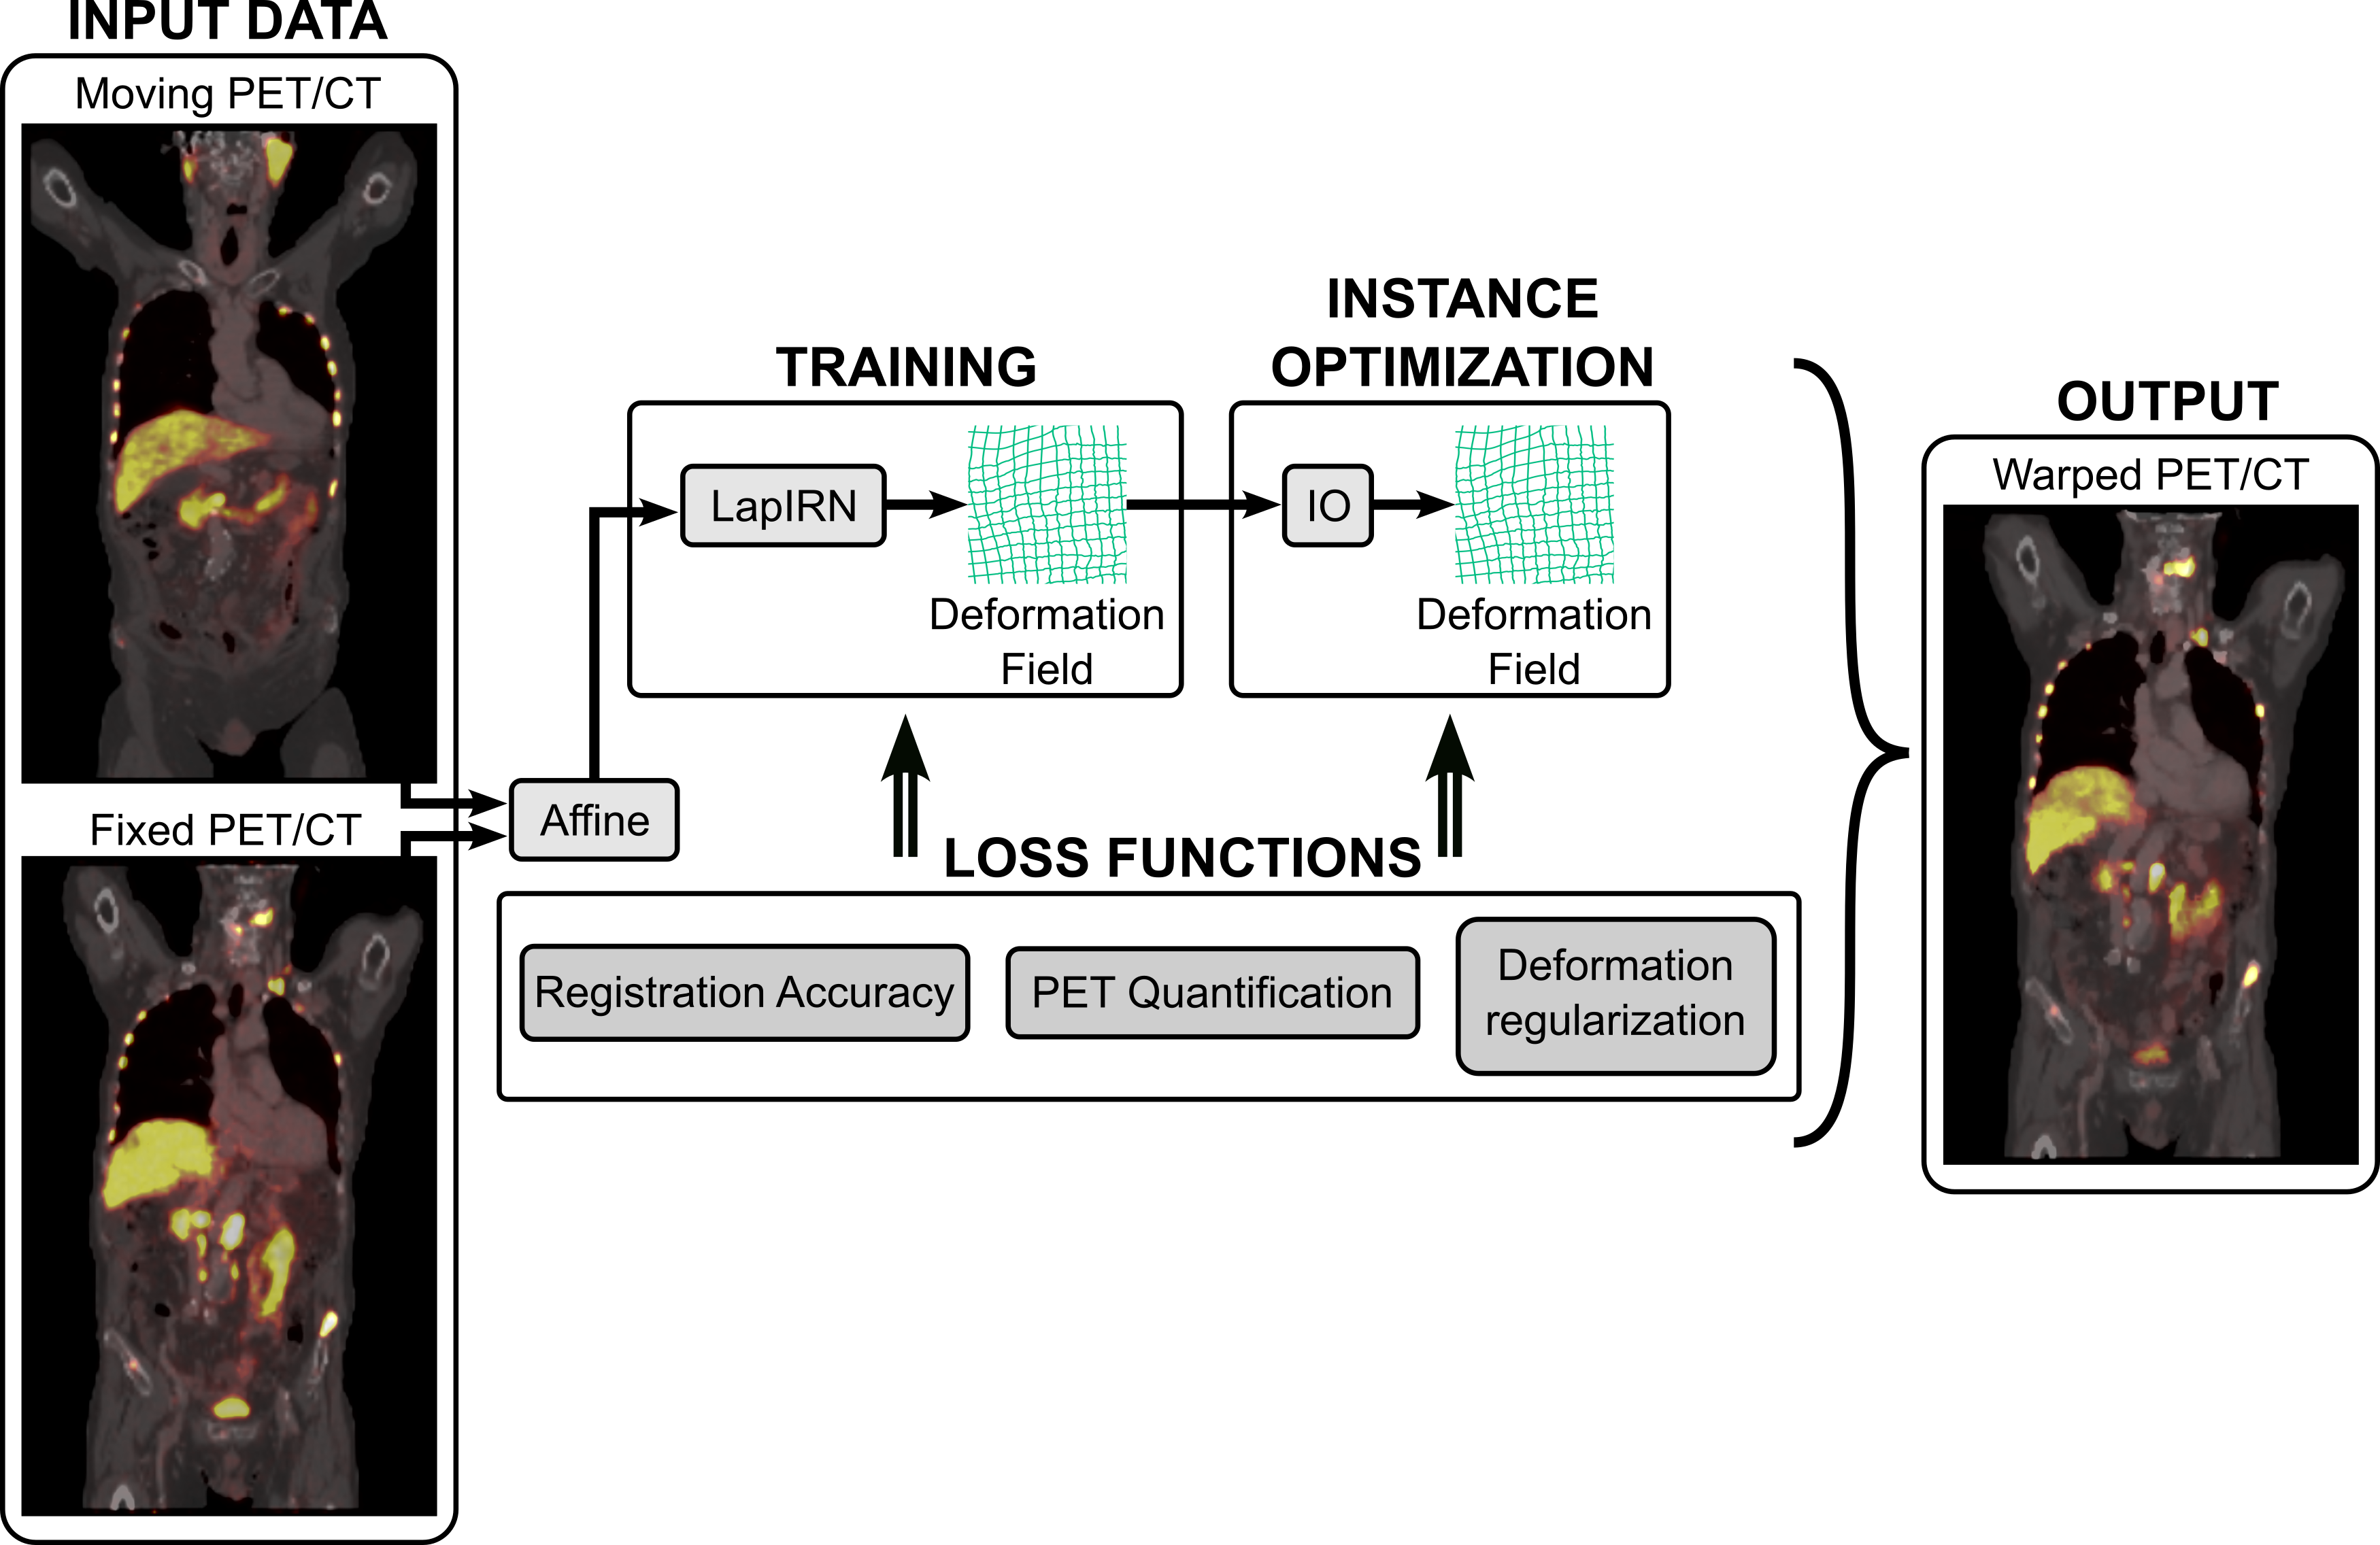
\includegraphics[width=\linewidth]{figures/overview.png}
\end{center}
\caption{\label{fig:pipeline}
Registration pipeline.
The follow-up (moving) and baseline (fixed) PET/CT images are aligned by an affine pre-registration, then by the LapIRN network, which predicts a dense deformation.
Instance optimization (IO) refines this deformation per pair before the moving image is resampled into the fixed frame.
Network training and IO use the same groups of loss terms: registration accuracy, bone rigidity, PET quantification, and deformation regularization (Sec.~\ref{sect:objective}).
The bone-rigidity and PET-quantification terms can be used in training, in IO, or in both; our method uses them only in IO.}
\end{figure}
